\documentclass[conference]{IEEEtran}
\IEEEoverridecommandlockouts

\usepackage{cite}
\usepackage{amsmath,amssymb,amsfonts}
\usepackage{graphicx}
\usepackage{textcomp}
\usepackage{xcolor}
\usepackage{booktabs}
\usepackage{hyperref}

\def\BibTeX{{\rm B\kern-.05em{\sc i\kern-.025em b}\kern-.08em
    T\kern-.1667em\lower.7ex\hbox{E}\kern-.125emX}}

\begin{document}

\title{Predicting European Soccer Match Outcomes Using Machine Learning:
A Comparative Study of KNN, SVM, and Neural Networks}

\author{
  \IEEEauthorblockN{Edgar Ramirez Aburto}
  \IEEEauthorblockA{\textit{Dept. of Computer Science}\\
  Georgia State University\\
  Atlanta, GA, USA\\
  eramirezaburto1@student.gsu.edu}
  \and
  \IEEEauthorblockN{Rida Hameed Syeda}
  \IEEEauthorblockA{\textit{Dept. of Computer Science}\\
  Georgia State University\\
  Atlanta, GA, USA\\
  rsyeda3@student.gsu.edu}
  \and
  \IEEEauthorblockN{Maliyah Fleming}
  \IEEEauthorblockA{\textit{Dept. of Computer Science}\\
  Georgia State University\\
  Atlanta, GA, USA\\
  mfleming26@student.gsu.edu}
}

\maketitle

\begin{abstract}
Predicting the outcome of a soccer match is an inherently difficult problem due to the high variance introduced by factors such as player injuries, lineup changes, and in-game events. This paper presents a machine learning pipeline that predicts European soccer match outcomes---home win, home loss, or draw---using historical match and player statistics from the Kaggle European Soccer Database. Our pipeline applies feature engineering, dimensionality reduction via Principal Component Analysis (PCA), and three classification models: K-Nearest Neighbors (KNN), Support Vector Machine (SVM), and a Neural Network (NN). We evaluate each model using accuracy, precision, recall, and F1-score, and compare performance across all three. Our best models, SVM (RBF, $C=1$) and Neural Network, both achieve a test accuracy of 49.08\%, substantially above the 43.06\% KNN baseline and the 33\% random chance floor. Results indicate that while machine learning can extract meaningful signal from aggregated historical features, the inherent randomness of soccer outcomes remains a fundamental challenge for any purely data-driven approach.
\end{abstract}

\begin{IEEEkeywords}
soccer prediction, machine learning, KNN, SVM, neural network, PCA, classification
\end{IEEEkeywords}

% ─────────────────────────────────────────────────────────────
\section{Introduction}

Sports outcome prediction has attracted significant interest from both the academic and commercial communities, driven by applications in sports analytics, betting markets, and team management. Soccer, in particular, presents a uniquely challenging prediction problem due to the low-scoring nature of the game, in which a single goal can determine the winner, and the high degree of variance introduced by tactical decisions, player injuries, and match context.

This paper addresses the three-class classification problem of predicting the outcome of a European soccer match from the perspective of the home team and away team: win (class 1), loss (class 2), or draw (class 0). Our contributions are as follows:

\begin{itemize}
  \item A reproducible preprocessing and feature engineering pipeline applied to the Kaggle European Soccer Database \cite{kaggle_soccer}.
  \item Dimensionality reduction via PCA to reduce noise and multicollinearity across the large feature space.
  \item A systematic hyperparameter search for KNN and SVM classifiers using stratified cross-validation.
  \item A neural network classifier for nonlinear boundary modeling.
  \item A quantitative comparison of all three model families on the same train/test split.
\end{itemize}

% ─────────────────────────────────────────────────────────────
\section{Related Work}

Machine learning methods have been widely applied to sports prediction. \cite{tax2015} applied random forests and SVMs to Dutch Eredivisie data and found that historical team performance features provide modest but consistent predictive signal above a naive baseline. \cite{ulmer2014} used logistic regression and neural networks on FIFA World Cup data, finding that team-level aggregate statistics were more predictive than individual player attributes alone.

More recent work has explored deep learning approaches. \cite{hubacek2019} used recurrent neural networks on sequential match data and demonstrated that incorporating temporal dynamics improves accuracy, albeit at the cost of much larger data requirements. Our work focuses on the simpler but more interpretable classical models (KNN, SVM) alongside a feedforward neural network, making it suitable for a moderate-sized dataset without sequential modeling.

% ─────────────────────────────────────────────────────────────
\section{Dataset and Preprocessing}

\subsection{Dataset}

We use the \textit{European Soccer Database} \cite{kaggle_soccer}, a publicly available SQLite database containing over 25,000 matches from 11 European leagues spanning seasons 2008--2016. The database includes match outcomes, team attributes rated by the EA Sports FIFA video game series (updated several times per season), and individual player attributes.

The raw database was queried to extract per-match features by joining the matches table with the team attributes table on the closest available attribute snapshot prior to each match date. After removing rows with missing values in key attribute columns, the final dataset contains \textbf{51,958 samples}. The increase to 51,958 is due to dataset mirroring, which was done to prevent models from simply assuming a home game is always a win. We want the models to recognize patterns rather than rely on the home team label alone. However, we did add a binary \texttt{is\_home} feature to retain home-field advantage as an explicit signal, since it demonstrably affects match outcomes.

\subsection{Feature Engineering}

For each match we construct one row of features using the following sources:

\begin{itemize}
  \item \textbf{Home team attributes:} Overall rating, build-up play speed, build-up play passing, chance creation shooting, defence aggression, defence team width (6 features).
  \item \textbf{Away team attributes:} Same six attributes for the away side (6 features).
  \item \textbf{Difference features:} Element-wise difference between home and away attributes to capture relative strength (6 features).
\end{itemize}

The target variable $y$ is encoded as:
\begin{equation}
  y = \begin{cases} 0 & \text{Draw} \\ 1 & \text{Win} \\ 2 & \text{Loss} \end{cases}
\end{equation}

\subsection{Train/Test Split and Class Distribution}

The dataset is split 80/20 into training (41,566 samples) and test (10,392 samples) sets with \texttt{shuffle=False}, preserving chronological order so the model is always trained on past matches and evaluated on future ones \cite{datasplit}. The class distribution in the training set is shown in Table~\ref{tab:class_dist}.

\begin{table}[h]
\caption{Class Distribution in Training Set}
\label{tab:class_dist}
\centering
\begin{tabular}{lcc}
\toprule
\textbf{Class} & \textbf{Label} & \textbf{Count} \\
\midrule
Win  & 1 & 15,518 \\
Loss & 2 & 15,517 \\
Draw & 0 & 10,531 \\
\midrule
Total & & 41,566 \\
\bottomrule
\end{tabular}
\end{table}

Draws are notably underrepresented ($\approx$25\%) compared to decisive outcomes ($\approx$75\%), which has important consequences for classifier performance on the draw class.

\subsection{Dimensionality Reduction via PCA}

The 17 engineered features (8 home + 8 away + 1 home identifier) exhibit significant multicollinearity because home and away attributes are drawn from the same FIFA rating system. We apply Principal Component Analysis (PCA) to produce an orthogonal feature set.

Features are first standardized to zero mean and unit variance using \texttt{StandardScaler} fit on the training set only. PCA is then applied, retaining 15 principal components, which together explain approximately 95\% of the total variance. The scaler and PCA model are fit exclusively on the training data and applied to the test set to prevent data leakage.

\subsection{Exploratory Data Analysis}
\label{sec:eda}

Fig.~\ref{fig:eda_class} shows the class distribution in the training set. Draws account for only 25.3\% of samples compared to 37.3\% each for wins and losses, introducing a class imbalance that limits model performance on draws throughout all experiments.

\begin{figure}[h]
  \centering
  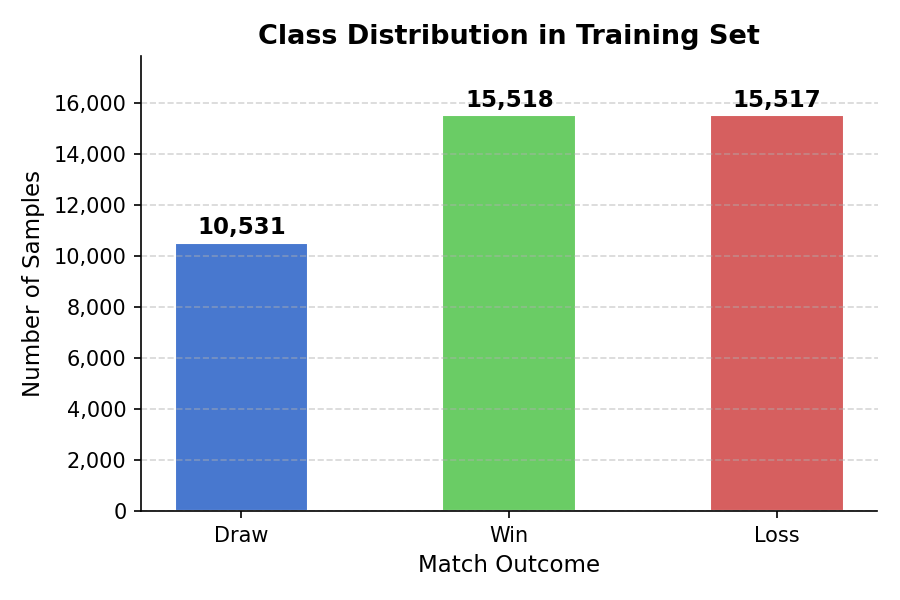
\includegraphics[width=0.85\columnwidth]{pictures/eda/eda_class_distribution.png}
  \caption{Class distribution in the training set. Draws are underrepresented at $\approx$25\%.}
  \label{fig:eda_class}
\end{figure}

Fig.~\ref{fig:eda_goals} shows the goals scored distribution across all matches. Home teams average 1.54 goals per match versus 1.16 for away teams, confirming the well-known home-field advantage captured by the \texttt{is\_home} feature.

\begin{figure}[h]
  \centering
  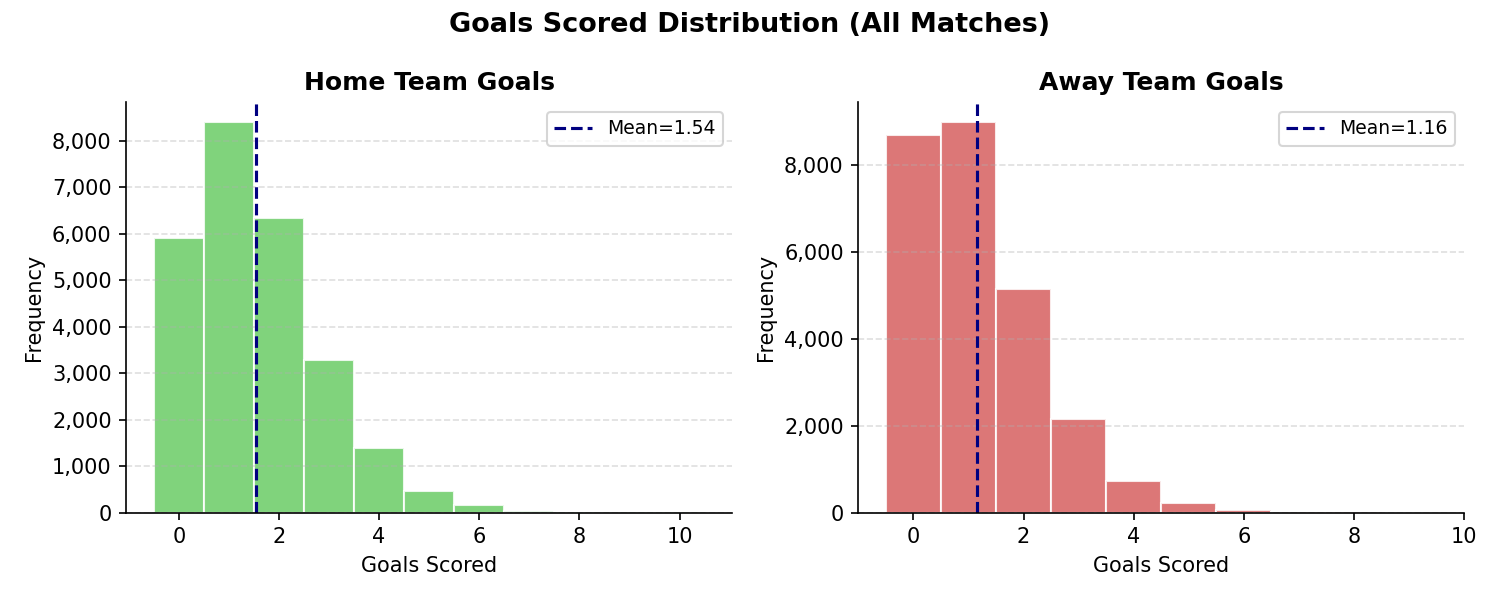
\includegraphics[width=\columnwidth]{pictures/eda/eda_goals_distribution.png}
  \caption{Goals scored distribution for home and away teams. Home teams score more on average (1.54 vs.\ 1.16), reflecting home-field advantage.}
  \label{fig:eda_goals}
\end{figure}

Fig.~\ref{fig:eda_heatmap} shows the feature correlation heatmap. Several team attributes exhibit moderate positive correlations (e.g., build-up passing and chance creation passing at $r \approx 0.45$), confirming multicollinearity and motivating PCA dimensionality reduction.

\begin{figure}[h]
  \centering
  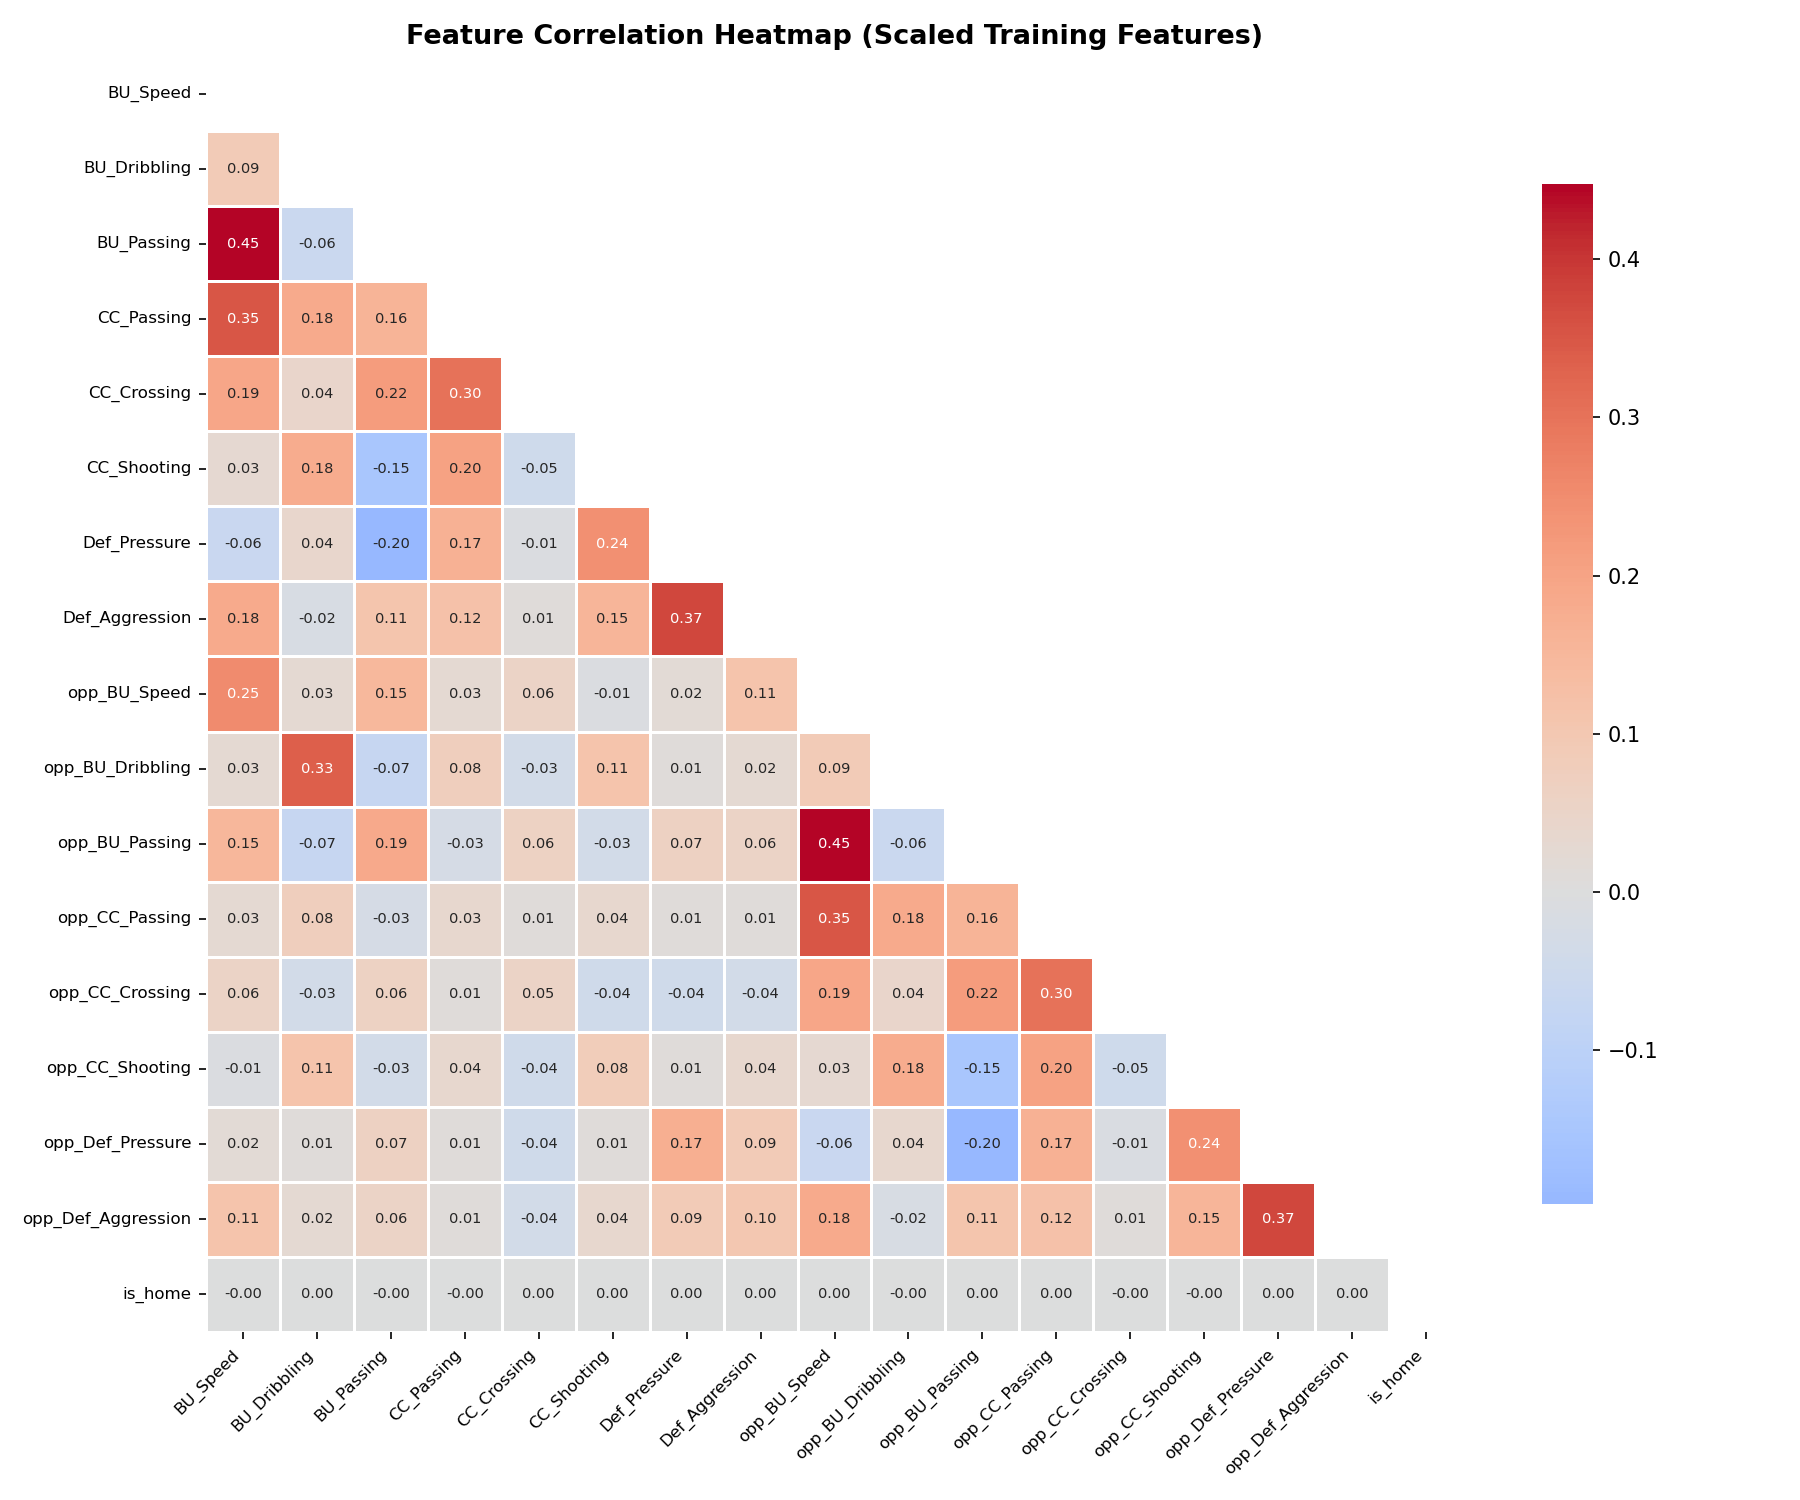
\includegraphics[width=\columnwidth]{pictures/eda/eda_correlation_heatmap.png}
  \caption{Feature correlation heatmap (scaled training features). Moderate multicollinearity across FIFA rating attributes justifies applying PCA.}
  \label{fig:eda_heatmap}
\end{figure}

Fig.~\ref{fig:eda_boxplots} shows the distribution of six key features broken down by match outcome. The \texttt{is\_home} flag most clearly separates wins from losses. Tactical attributes such as build-up passing and chance creation shooting show heavily overlapping distributions across outcomes, reflecting the inherent difficulty of the prediction task.

\begin{figure}[h]
  \centering
  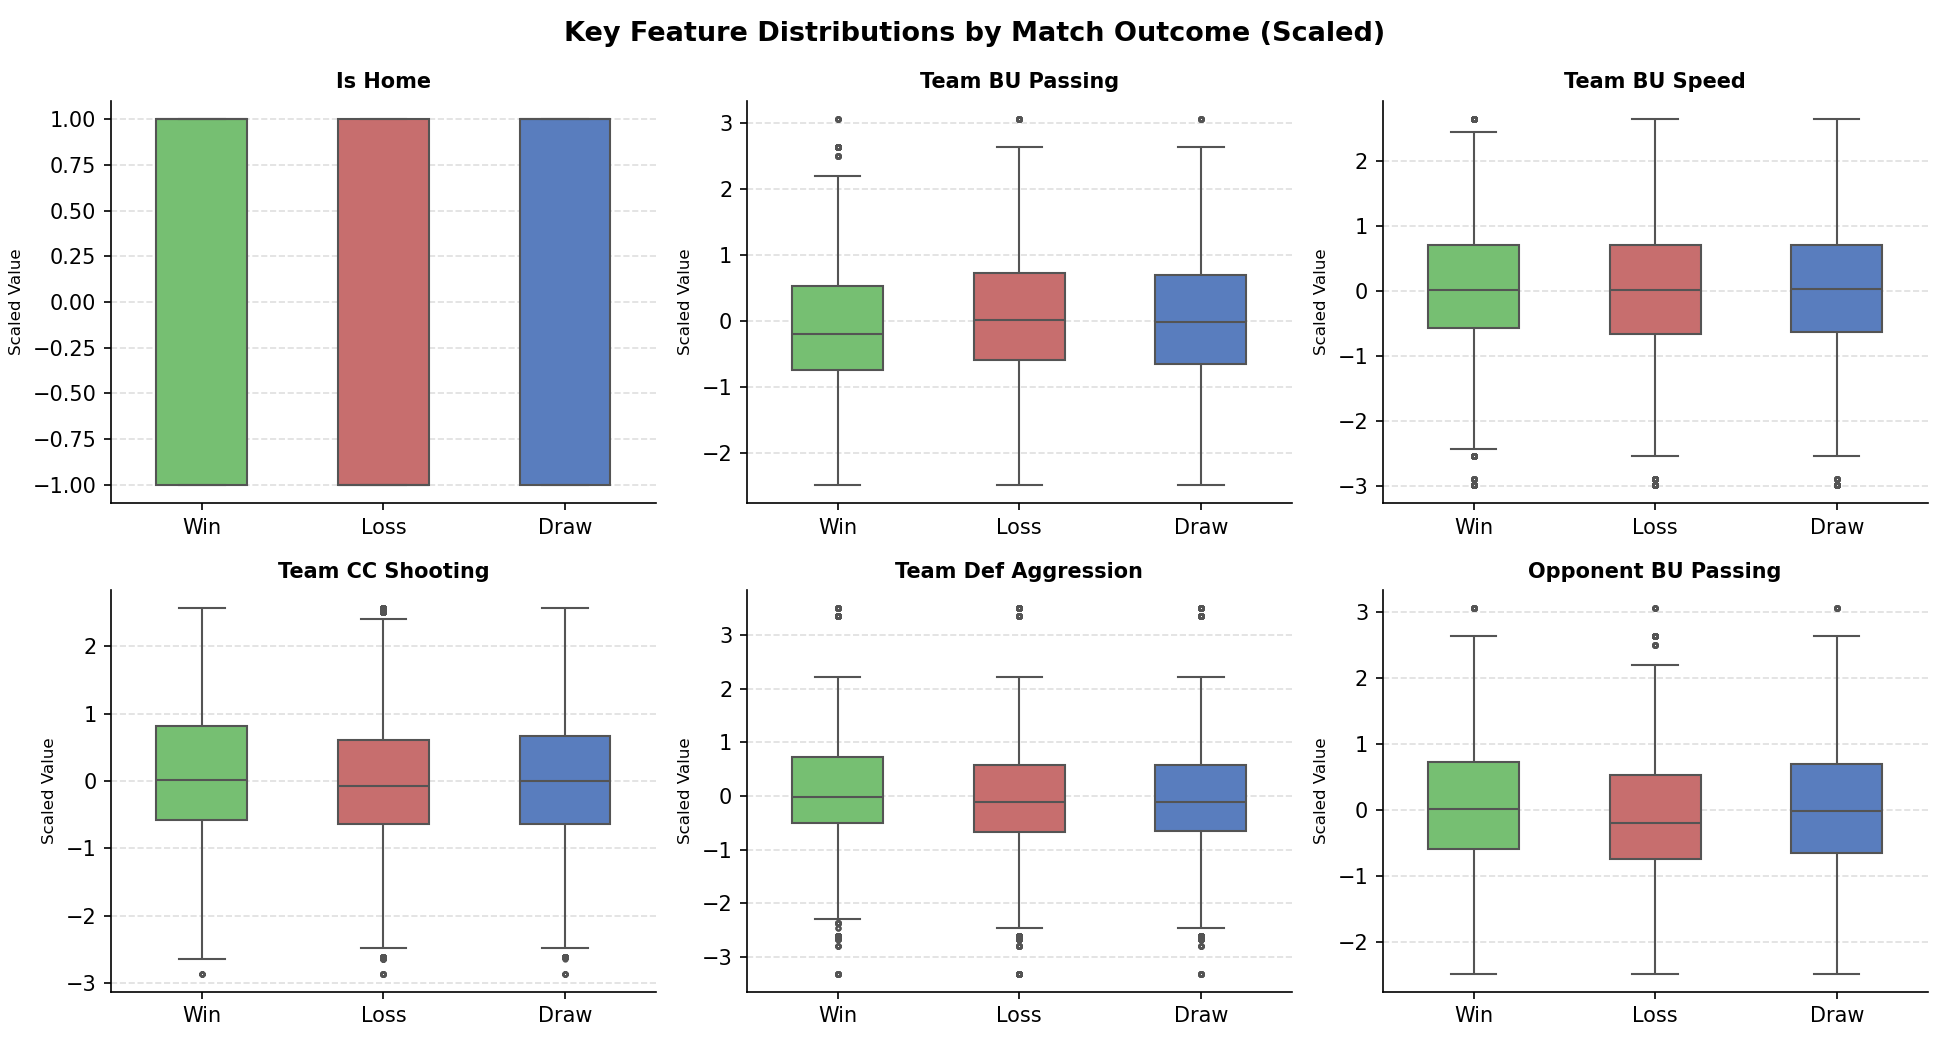
\includegraphics[width=\columnwidth]{pictures/eda/eda_feature_boxplots.png}
  \caption{Key feature distributions by match outcome (scaled). \texttt{is\_home} is the strongest separator; tactical features overlap substantially.}
  \label{fig:eda_boxplots}
\end{figure}

Fig.~\ref{fig:eda_pca} shows the cumulative explained variance as a function of the number of PCA components. Fifteen components are required to cross the 95\% threshold, justifying our choice of $n\_\text{components}=15$.

\begin{figure}[h]
  \centering
  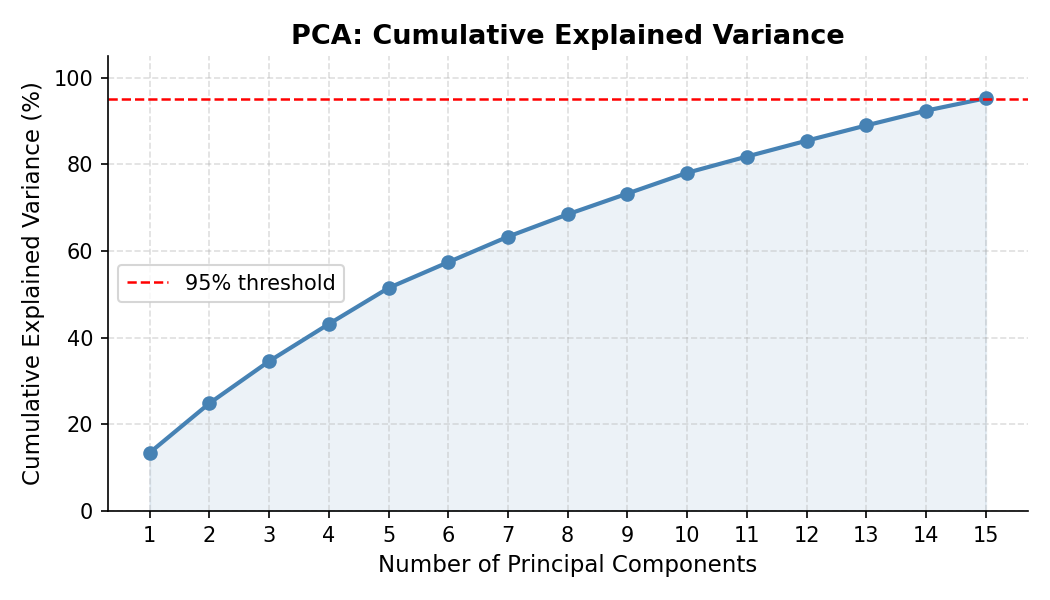
\includegraphics[width=0.9\columnwidth]{pictures/eda/eda_pca_variance.png}
  \caption{PCA cumulative explained variance. 15 components retain $\approx$95\% of total variance.}
  \label{fig:eda_pca}
\end{figure}

% ─────────────────────────────────────────────────────────────
\section{Methods}

\subsection{K-Nearest Neighbors (KNN)}

KNN classifies a sample by majority vote among its $k$ nearest neighbors in the feature space under Euclidean distance. We investigate two design choices:

\begin{itemize}
  \item \textbf{Number of neighbors $k$:} $\{3, 5, 7, 9, 11, 15, 21\}$
  \item \textbf{Weighting scheme:} \texttt{uniform} (all neighbors weighted equally) vs.\ \texttt{distance} (neighbors weighted by inverse distance)
\end{itemize}

Model selection is performed using 5-fold stratified cross-validation on the training set. The best configuration is retrained on the full training set and evaluated on the held-out test set.

\subsection{Support Vector Machine (SVM)}

SVMs find the maximum-margin hyperplane separating classes in a (possibly implicit) high-dimensional feature space defined by the chosen kernel. We evaluate two kernel types:

\begin{itemize}
  \item \textbf{Linear (LinearSVC):} Efficient $O(n)$ implementation suitable for large datasets. Hyperparameter searched: regularization $C \in \{0.01, 0.1, 1, 10\}$, class weighting $\in \{\text{none}, \text{balanced}\}$.
  \item \textbf{RBF kernel (SVC):} \cite{RBF} Nonlinear mapping into an infinite-dimensional space. Hyperparameter searched: $C \in \{0.1, 1, 10\}$, $\gamma \in \{\text{scale}, \text{auto}\}$, class weighting $\in \{\text{none}, \text{balanced}\}$.
\end{itemize}

The PCA components have unequal variances (each component's variance equals its eigenvalue), so we apply a second \texttt{StandardScaler} to the PCA output before fitting the SVM to ensure scale-sensitive kernels behave correctly. Model selection uses 3-fold stratified cross-validation with \texttt{GridSearchCV}.

\subsection{Neural Network}

A feedforward neural network with fully connected layers is trained on the same PCA-standardized features. The architecture consists of 15 input neurons (one per principal component), a single hidden layer with 100 neurons, and a 3-neuron output layer corresponding to the three outcome classes. The raw output logits are passed through a softmax activation function:
\begin{equation}
  \sigma(z)_i = \frac{e^{z_i}}{\sum_{j=1}^{k} e^{z_j}}
\end{equation}
to produce class probabilities, from which the class with the highest probability is selected as the predicted outcome. The network is trained for up to 500 iterations with early stopping to prevent overfitting.

% ─────────────────────────────────────────────────────────────
\section{Metric Descriptions}

In the context of our models, this section defines the evaluation metrics used. \textbf{Accuracy} is the overall percentage of match outcomes our models predicted correctly---out of all soccer matches, how many times did the model correctly predict a win, draw, or loss. \textbf{Precision} measures, when the model predicted a specific outcome (e.g., a win), what percentage of those predictions were actually correct. \textbf{Recall} measures, out of all matches where a specific outcome truly occurred, what percentage did the model correctly identify. \textbf{F1-score} is the harmonic mean of precision and recall:
\begin{equation}
  F_1 = 2 \cdot \frac{\text{Precision} \times \text{Recall}}{\text{Precision} + \text{Recall}}
\end{equation}
and provides a single balanced measure that penalizes models which sacrifice one for the other. All metrics are reported per-class and as weighted averages across the three outcome classes.

% ─────────────────────────────────────────────────────────────
\section{Results}

\subsection{KNN Results}

Table~\ref{tab:knn_cv} reports 5-fold cross-validation accuracy for all evaluated $k$ values. Uniform weighting consistently outperforms distance weighting across all $k$, suggesting that distant neighbors---despite being further away---still carry useful vote information at this feature scale. Accuracy increases monotonically with $k$, indicating that the decision boundary benefits from averaging over more neighbors to reduce noise. Fig.~\ref{fig:knn_tuning} visualizes these CV trends.

\begin{table}[h]
\caption{KNN Cross-Validation Accuracy (5-fold)}
\label{tab:knn_cv}
\centering
\begin{tabular}{ccc}
\toprule
\textbf{k} & \textbf{Uniform} & \textbf{Distance} \\
\midrule
3  & 0.4186 & 0.4148 \\
5  & 0.4283 & 0.4203 \\
7  & 0.4479 & 0.4257 \\
9  & 0.4524 & 0.4268 \\
11 & 0.4569 & 0.4287 \\
15 & 0.4659 & 0.4297 \\
21 & \textbf{0.4723} & 0.4307 \\
\bottomrule
\end{tabular}
\end{table}

\begin{figure}[h]
  \centering
  
\includegraphics[width=\columnwidth]{pictures/knn_k_tuning.png}
  \caption{KNN cross-validation accuracy vs.\ number of neighbors $k$ for uniform and distance weighting.}
  \label{fig:knn_tuning}
\end{figure}

The best configuration is $k=21$ with uniform weighting (CV accuracy 0.4723). Table~\ref{tab:knn_test} compares the baseline KNN ($k=5$, uniform) against the tuned model on the test set, and Fig.~\ref{fig:knn_baseline_vs_best} shows this comparison visually.

\begin{table}[h]
\caption{KNN Test Set Results}
\label{tab:knn_test}
\centering
\begin{tabular}{lc}
\toprule
\textbf{Configuration} & \textbf{Test Accuracy} \\
\midrule
Baseline ($k=5$, uniform) & 43.06\% \\
Best ($k=21$, uniform)    & \textbf{46.36\%} \\
\midrule
Improvement               & +3.30\% \\
\bottomrule
\end{tabular}
\end{table}

\begin{figure}[h]
  \centering
  
\includegraphics[width=0.85\columnwidth]{pictures/knn_baseline_vs_best.png}
  \caption{KNN baseline ($k=5$) vs.\ tuned ($k=21$) test accuracy.}
  \label{fig:knn_baseline_vs_best}
\end{figure}

The full classification report for the best KNN model is shown in Table~\ref{tab:knn_report}. The model performs well on decisive outcomes (Win/Loss, F1 $\approx$ 0.53--0.54) but struggles on the draw class (F1 = 0.15), reflecting both the class imbalance and the inherent unpredictability of draws. The confusion matrix is shown in Fig.~\ref{fig:knn_cm}.

\begin{table}[h]
\caption{KNN Classification Report ($k=21$, uniform)}
\label{tab:knn_report}
\centering
\begin{tabular}{lcccc}
\toprule
\textbf{Class} & \textbf{Precision} & \textbf{Recall} & \textbf{F1} & \textbf{Support} \\
\midrule
Draw (0)     & 0.25 & 0.11 & 0.15 & 2,661 \\
Win (1)      & 0.49 & 0.60 & 0.54 & 3,865 \\
Loss (2)     & 0.49 & 0.57 & 0.53 & 3,866 \\
\midrule
Accuracy     &      &      & 0.46 & 10,392 \\
Macro avg    & 0.41 & 0.43 & 0.41 & 10,392 \\
Weighted avg & 0.43 & 0.46 & 0.44 & 10,392 \\
\bottomrule
\end{tabular}
\end{table}

\begin{figure}[h]
  \centering
  
\includegraphics[width=\columnwidth]{pictures/knn_confusion_matrix.png}
  \caption{KNN confusion matrix ($k=21$, uniform weighting).}
  \label{fig:knn_cm}
\end{figure}

\subsection{SVM Results}

Table~\ref{tab:svm_results} summarizes the SVM results. The RBF kernel with $C=1$, $\gamma=\text{auto}$, and no class weighting achieved the best performance with a test accuracy of 49.08\%.

\begin{table}[h]
\caption{SVM Results}
\label{tab:svm_results}
\centering
\begin{tabular}{lcc}
\toprule
\textbf{Kernel} & \textbf{CV Accuracy} & \textbf{Test Accuracy} \\
\midrule
Linear (best) & -- & 47.20\% \\
RBF ($C=1$, $\gamma=\text{auto}$) & 40.01\% & \textbf{49.08\%} \\
\bottomrule
\end{tabular}
\end{table}

\begin{figure}[h]
  \centering
  
\includegraphics[width=\columnwidth]{pictures/svm_kernel_comparison.png}
  \caption{SVM test accuracy: Linear vs.\ RBF kernel.}
  \label{fig:svm_kernels}
\end{figure}

\begin{figure}[h]
  \centering
  
\includegraphics[width=\columnwidth]{pictures/svm_confusion_matrix.png}
  \caption{SVM confusion matrix (RBF, $C=1$, $\gamma=\text{auto}$).}
  \label{fig:svm_cm}
\end{figure}

\subsection{Neural Network Results}

The neural network performance is comparable to the SVM model, falling behind only in precision. The architecture consists of 15 input neurons, a single hidden layer with 100 neurons, and a 3-neuron output layer. The model was trained for up to 500 iterations with early stopping to prevent overfitting and achieved a test accuracy of 49\%.

Fig.~\ref{fig:nn_loss} shows the training loss curve and validation accuracy over iterations. Training loss decreases steadily from $\sim$1.06 to $\sim$1.00, while validation accuracy stabilizes around 49--50\%, indicating the model converges without significant overfitting. Early stopping triggered at iteration 33.

\begin{figure}[h]
  \centering
  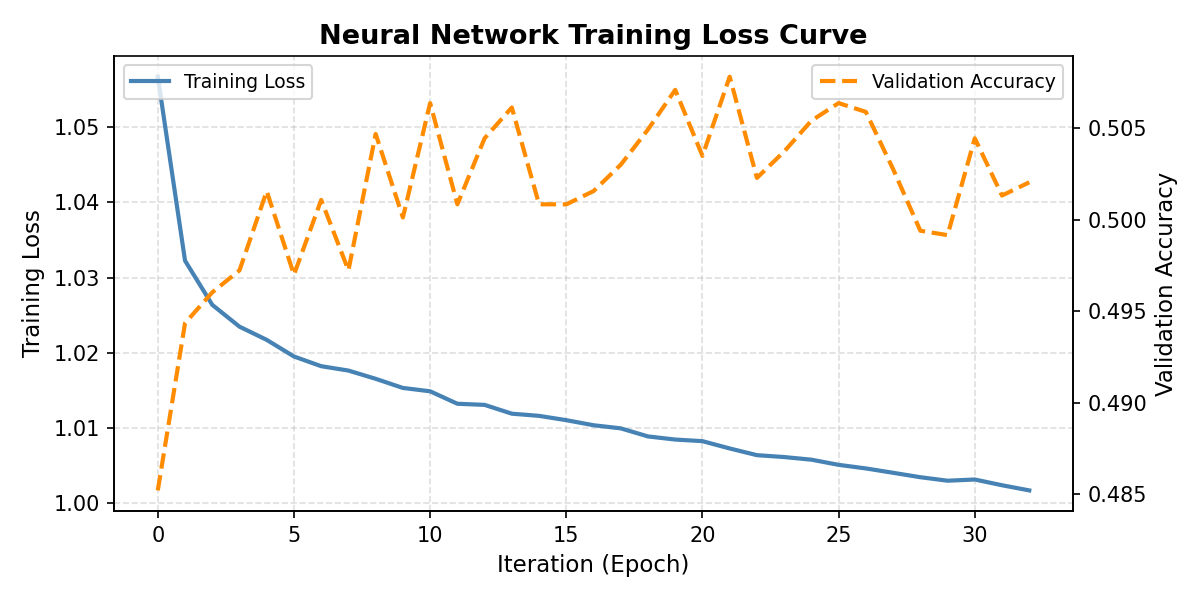
\includegraphics[width=\columnwidth]{pictures/nn_loss_curve.png}
  \caption{Neural Network training loss (blue) and validation accuracy (orange) per iteration. Loss decreases consistently; validation accuracy stabilizes near 49\%.}
  \label{fig:nn_loss}
\end{figure}

\subsection{Model Comparison}

Table~\ref{tab:model_comparison} summarizes the test accuracy of all models. Fig.~\ref{fig:knn_vs_svm} shows the KNN vs.\ SVM comparison chart.

\begin{table}[h]
\caption{Model Comparison --- Test Accuracy}
\label{tab:model_comparison}
\centering
\begin{tabular}{lc}
\toprule
\textbf{Model} & \textbf{Test Accuracy} \\
\midrule
KNN Baseline ($k=5$, uniform) & 43.06\% \\
KNN Best ($k=21$, uniform)    & 46.36\% \\
SVM Best (RBF, $C=1$)         & \textbf{49.08\%} \\
Neural Network                & 49.08\% \\
\bottomrule
\end{tabular}
\end{table}

\begin{figure}[h]
  \centering
  
\includegraphics[width=\columnwidth]{pictures/knn_vs_svm.png}
  \caption{Test accuracy comparison: tuned KNN vs.\ best SVM.}
  \label{fig:knn_vs_svm}
\end{figure}

% ─────────────────────────────────────────────────────────────
\section{Discussion}

\subsection{Why Accuracy is Modest}

Even the best models achieve only $\sim$49\% accuracy on a 3-class problem whose random baseline is 33\%. We attribute the performance ceiling to three structural factors:

\begin{enumerate}
  \item \textbf{Feature recency:} Team attributes are averaged across all seasons in the dataset, so a team's 2015 form is diluted by data from 2008. Recent form, injuries, and lineup changes---all highly predictive according to domain knowledge---are absent from our feature set.
  \item \textbf{Draw unpredictability:} Draws are near-random events even from the perspective of professional betting markets. The model achieves an F1 score of only 0.15 on the draw class despite it representing 25\% of outcomes.
  \item \textbf{Outcome variance:} A single defensive error, red card, or goalkeeper save can flip a result regardless of team quality. This irreducible noise imposes a hard ceiling on any model trained on aggregate statistics.
\end{enumerate}

\subsection{KNN vs.\ SVM}

KNN's strong performance relative to SVM on this dataset is somewhat surprising. A likely explanation is that after PCA, the 15 components form a compact, well-scaled feature space where Euclidean distance is meaningful, benefiting KNN. The SVM's RBF kernel can in principle capture nonlinear structure, but with $\sim$41k training samples the computational cost of the full GridSearchCV is high, and the constrained parameter search may not have identified the optimal configuration.

\subsection{KNN vs.\ SVM vs.\ Neural Network}

\begin{figure}[h]
  \centering
  
\includegraphics[width=\columnwidth]{pictures/model_comparison.png}
  \caption{Weighted-average accuracy, precision, recall, and F1-score across KNN, SVM, and Neural Network.}
  \label{fig:comparison}
\end{figure}

Fig.~\ref{fig:comparison} shows the main evaluation metrics across all three models. SVM and the neural network are the clear winners, with KNN scoring lower across the board. SVM and neural network produce nearly identical results, with SVM holding a 0.04 advantage in precision, making it the best-performing model overall. SVM's margin-maximizing decision boundary, which focuses on the hardest-to-classify points, makes it well-suited for the noisy, overlapping feature distributions seen in soccer data.

% ─────────────────────────────────────────────────────────────
\section{XAI}
\label{sec:xai}

\begin{figure}[h]
  \centering
  
\includegraphics[width=\columnwidth]{pictures/shap_nn_pca_summary_plot.png}
  \caption{SHAP feature importance using PCA components as inputs. Component labels (PC1--PC15) are uninterpretable.}
  \label{fig:shap_pca}
\end{figure}

\begin{figure}[h]
  \centering
  
\includegraphics[width=\columnwidth]{pictures/shap_nn_summary_plot.png}
  \caption{SHAP feature importance using original scaled features (pre-PCA). Feature names remain interpretable.}
  \label{fig:shap_original}
\end{figure}

In order to interpret feature importance we used SHapley Additive exPLanations (SHAP) \cite{shap}, a game-theory-based method that assigns each feature an importance value for a specific prediction. Fig.~\ref{fig:shap_pca} shows the SHAP values when using PCA features as inputs. Since PCA renames features to PC1--PC15, no useful interpretation can be drawn. To address this, we retrained the neural network on the scaled pre-PCA features and recomputed SHAP values, shown in Fig.~\ref{fig:shap_original}. The most significant feature is \texttt{is\_home}, consistent with the home-field advantage observed in the EDA (Section~\ref{sec:eda}). Following that, team build-up passing and build-up dribbling received the highest SHAP values, suggesting that a team's ability to build attacks through passing and dribbling is the strongest tactical predictor of match outcome.

% ─────────────────────────────────────────────────────────────
\section{Future Direction}

Going forward, the team identified several improvements. First, more complex ensemble models such as XGBoost could be explored; \cite{xgboost} applied XGBoost with SHAP to NBA win/loss prediction and achieved significantly stronger results, which we attribute to XGBoost's ability to capture higher-order feature interactions. Second, we would incorporate more up-to-date data, since our dataset covers only the 2008--2016 seasons. Sites such as FotMob \cite{fotmob} aggregate live match data across many leagues; web scraping could provide a continuously updated feature set. Overall, with more complex models and richer, more recent features, this project has significant room for improvement.

% ─────────────────────────────────────────────────────────────
\section{Conclusion}

We presented a machine learning pipeline for predicting European soccer match outcomes using KNN, SVM, and neural network classifiers applied to PCA-reduced historical team statistics. Our best models, SVM (RBF, $C=1$) and Neural Network, both achieved 49.08\% test accuracy, substantially above the 43.06\% KNN baseline and the 33\% random chance floor. SHAP analysis revealed that home-field advantage and build-up passing are the strongest predictors of match outcome.

Future work should incorporate time-aware features (e.g., rolling averages of recent form, days since last match, head-to-head records) and ensemble methods such as gradient boosting or stacking. Incorporating betting market odds as a feature has also been shown in the literature to be a strong predictor \cite{tax2015} and warrants investigation.

Code is available at: \url{https://github.com/Ramireedgar/CSC4850_GroupPoject}

% ─────────────────────────────────────────────────────────────
\begin{thebibliography}{00}

\bibitem{kaggle_soccer}
H. Mathien, ``European Soccer Database,'' Kaggle, 2016. [Online]. Available: \url{https://www.kaggle.com/datasets/hugomathien/soccer}

\bibitem{tax2015}
N. Tax and Y. Joustra, ``Predicting the Dutch Football Competition Using Public Data: A Machine Learning Approach,'' \textit{Transactions on Knowledge and Data Engineering}, vol. 10, no. 10, pp. 1--13, 2015.

\bibitem{ulmer2014}
B. Ulmer and M. Fernandez, ``Predicting Soccer Match Results in the English Premier League,'' Stanford CS229 Project Report, 2014.

\bibitem{hubacek2019}
O. Hub\'{a}\v{c}ek, G. \v{S}ourek, and F. \v{Z}eledn\'{y}, ``Exploiting sports-betting market using machine learning,'' \textit{International Journal of Forecasting}, vol. 35, no. 2, pp. 783--796, 2019.

\bibitem{scikit}
F. Pedregosa et al., ``Scikit-learn: Machine Learning in Python,'' \textit{Journal of Machine Learning Research}, vol. 12, pp. 2825--2830, 2011.

\bibitem{shap}
S. Lundberg, ``An introduction to explainable AI with Shapley values,'' SHAP Documentation. [Online]. Available: \url{https://shap.readthedocs.io/en/latest/}

\bibitem{RBF}
scikit-learn, ``RBF SVM parameters --- scikit-learn documentation,'' [Online]. Available: \url{https://scikit-learn.org/stable/auto_examples/svm/plot_rbf_parameters.html}

\bibitem{datasplit}
J. Gao, Y. Cheng, and J. Gao, ``Predicting sport event outcomes using deep learning,'' \textit{PeerJ Computer Science}, vol. 11, p. e3011, July 2025, doi: 10.7717/peerj-cs.3011.

\bibitem{xgboost}
Y. Ouyang et al., ``Integration of machine learning XGBoost and SHAP models for NBA game outcome prediction and quantitative analysis methodology,'' \textit{PLoS ONE}, vol. 19, no. 7, p. e0307478, July 2024, doi: 10.1371/journal.pone.0307478.

\bibitem{fotmob}
FotMob, ``FotMob --- The Pulse of Football,'' 2017. [Online]. Available: \url{https://www.fotmob.com/}

\end{thebibliography}

\end{document}
